\documentclass[preprint,12pt]{elsarticle}

\usepackage{amsmath,amssymb,amsthm}
\usepackage{graphicx}
\usepackage{booktabs}
\usepackage{hyperref}
\usepackage{xcolor}
\usepackage{multirow}
\usepackage{microtype}
\usepackage{lineno}

\modulolinenumbers[5]

\journal{Neural Networks}

\graphicspath{{../analysis/figures/}}

\newtheorem{proof-sketch}{Proof Sketch}

\begin{frontmatter}

\title{When Does Gated Hybrid Memory Help? A Mechanistic Study of Layerwise Gamma Scheduling and Scalar-Gated Engram in Retentive Networks}

\author[inst1]{Author\corref{cor1}}
\cortext[cor1]{Corresponding author}
\ead{author@institution.edu}
\institute[inst1]{Institution, City, Country}

\begin{abstract}
We present a controlled mechanistic study of two augmentations to Retentive Networks (RetNet) for small-scale language modeling: \textbf{layerwise gamma scheduling} (depth-dependent retention decay, zero additional parameters) and \textbf{scalar-gated Engram hash tables} (O(1) N-gram lookup). Rather than proposing a novel architecture, we systematically decompose \emph{when and why} each component helps, and---critically---when it does not.

On Shakespeare char-level modeling (d=128, lr=$10^{-3}$, seed=42), layerwise gamma drives the scaling advantage: RetNet+layerwise improves from +4.3\% (losing to Transformer at 5K) to -20.9\% (winning at 20K), with a scaling law exponent 1.7$\times$ steeper than Transformer ($b{=}-0.495$ vs $-0.294$). Engram provides a stable $\sim$27\% acceleration at d=128 but exhibits a \emph{training-duration-dependent} effect at d=256: it hurts by +22.8\% at 5K steps before becoming beneficial (-3.1\%) at 20K---the scalar gate requires sufficient optimization to filter hash collisions at larger model widths.

We identify clear failure modes: Engram is unreliable on BPE tokenization (std=11.4 vs Transformer std=3.3) and on repetitive data where Transformer catches up. The advantage is dataset-dependent: growing on diverse data (Shakespeare: -42.4\% at 20K) but reversing on repetitive data (TinyStories: +14.9\% at 10K). A contrastive chunk retrieval pipeline extends context to 1M tokens on a synthetic needle-in-a-haystack task (EM=1.000). All findings are validated with multi-seed experiments and complete ablation studies.
\end{abstract}

\begin{keyword}
Retentive Network \sep language modeling \sep gated memory \sep scaling laws \sep mechanistic study
\end{keyword}

\end{frontmatter}

\linenumbers

\section{Introduction}
\label{sec:intro}

Small dense language models face a tension: attention scales quadratically, while linear alternatives sacrifice quality. Retentive Networks (RetNet)~\citep{sun2023retnet} offer a promising middle ground with O(1) recurrent inference, but their default configuration leaves room for improvement. Two natural augmentations arise: (1) allowing the retention decay parameter $\gamma$ to vary across layers, and (2) augmenting recurrent states with external memory lookups.

However, existing work lacks a systematic understanding of \emph{when these augmentations help, how they interact, and when they fail}. We address this gap through controlled experiments that decompose each component's contribution across model sizes, training durations, datasets, and tokenization schemes.

Our contributions are primarily \textbf{empirical and diagnostic}:

\begin{enumerate}
\item \textbf{Layerwise gamma is the scaling driver.} Depth-dependent retention decay costs zero parameters yet yields a scaling law exponent 1.7$\times$ steeper than Transformer, explaining the growing advantage with training duration.

\item \textbf{Engram is conditionally beneficial.} At d=128, scalar-gated Engram hash tables provide a stable $\sim$27\% acceleration. At d=256, the effect is training-duration-dependent: Engram hurts early (+22.8\% at 5K) before becoming beneficial (-3.1\% at 20K), revealing a gate convergence requirement at larger model widths.

\item \textbf{Advantage scales with data diversity.} On diverse data (Shakespeare), the advantage grows monotonically from -20.8\% (5K) to -42.4\% (20K). On repetitive data (TinyStories), Transformer catches up and reverses the advantage. This suggests gated memory is most valuable in compute-limited settings on diverse corpora.

\item \textbf{Clear failure modes.} Engram is unreliable on BPE tokenization (initialization-dependent variance), hurts on repetitive data given sufficient training, and requires gate convergence at large model widths. A contrastive chunk retrieval pipeline achieves EM=1.000 on synthetic needle-in-a-haystack at 1M tokens, but this is a controlled diagnostic rather than a real-world benchmark.
\end{enumerate}

We call the combined system \textbf{Anamnesis} (RetNet + layerwise gamma + scalar-gated Engram + chunk retrieval), but emphasize that our primary contribution is the mechanistic decomposition rather than the architecture itself.

\section{Related Work}
\label{sec:related}

\textbf{Efficient sequence models.} Transformer~\citep{vaswani2017attention} achieves strong quality but $O(N^2)$ attention. Linear Attention~\citep{katharopoulos2020linear} reduces to $O(N)$ via kernelized feature maps but sacrifices expressivity (10.39 vs 5.12 PPL in our controlled comparison). RetNet~\citep{sun2023retnet} achieves both parallel training and $O(1)$ recurrent inference via retention, forming our backbone. Mamba~\citep{gu2023mamba} uses selective state-space models with input-dependent parameters; our layerwise gamma provides a simpler, parameter-free form of temporal specialization. In our controlled comparison at seq\_len=128, Mamba achieves PPL=3.77 vs Anamnesis 5.53 (same 1000 steps), suggesting SSMs excel at short context. At seq\_len=512, Anamnesis achieves 3.12 PPL (5K steps), benefiting from longer context windows that Engram hash tables exploit. Gated DeltaNet~\citep{deltanet2025} proposes a delta update rule for key-value stores; our TokenCopyBuffer provides exact recall without learned updates.

\textbf{Memory-augmented networks.} External memory tables have a long history in neural networks~\citep{mcclelland1995cls,tonegawa2015engram}. Conditional Memory via Scalable Lookup~\citep{cheng2026conditionalmemory} proposes learnable retrieval from static key-value stores. Our Engram hash tables differ in using scalar gating~(Section~\ref{sec:engram}) and N-gram hashing~\citep{weinberger2009featurehashing} for O(1) lookup, with collision analysis via Count-Min sketch theory~\citep{cormode2005countmin}. Unlike attention-based memory~\citep{wu2022memorizing}, Engram requires no softmax or normalization---the gate directly controls injection strength.

\textbf{Scaling laws.} Prior work has established power-law scaling for Transformer language models. We extend this analysis to RetNet-based architectures, finding a 1.7$\times$ steeper scaling exponent that quantitatively explains the growing advantage with training duration.

\section{Method}
\label{sec:method}

\subsection{RetNet with Layerwise Gamma}
\label{sec:retnet}

RetNet's retention mechanism computes:
\begin{equation}
\text{Ret}(\mathbf{X}) = \text{softmax}(\mathbf{Q}\mathbf{K}^T / \sqrt{d}) \odot \gamma \mathbf{V}
\end{equation}
where $\gamma \in (0, 1)$ is a decay parameter. The original RetNet uses a \emph{single} $\gamma$ for all layers. We propose \textbf{layerwise gamma}: assigning each layer $l$ a distinct $\gamma_l$, scheduled as:
\begin{equation}
\gamma_l = \gamma_{\min} + (\gamma_{\max} - \gamma_{\min}) \cdot \frac{l}{L-1}
\end{equation}
where $L$ is the number of layers. This requires \textbf{zero additional parameters}---$\gamma$ is already present in RetNet, we simply unshare it across layers. The intuition: early layers should retain less (capturing local patterns), while deeper layers should retain more (accumulating global context). The spread $(\gamma_{\max} - \gamma_{\min})$ is optimized via grid search (U-shaped optimum at spread=1.0).

\subsection{Scalar-Gated Engram Hash Tables}
\label{sec:engram}

Engram stores recent N-gram statistics in fixed-size hash tables:
\begin{equation}
\mathbf{h} = \text{HashTable}[\text{hash}(\mathbf{x}_{t-n:t})]
\end{equation}
\begin{equation}
\mathbf{y} = g \cdot \mathbf{h}, \quad g = \sigma(\mathbf{w}^T \mathbf{x}_t + b)
\end{equation}
where $g \in (0,1)$ is a learned scalar gate. We use \textbf{scalar} rather than vector gating because scalar gating preserves the direction of $\mathbf{h}$ in embedding space (Proof~40 in Appendix), yielding +3\% PPL improvement over vector gating.

Key design: the gate $g$ is critical---without it, hash collisions inject noise. At small model widths (d=128), the gate converges quickly. At larger widths (d=256), the gate requires more training to distinguish signal from collision noise, explaining the time-dependent effect we observe.

\subsection{O(1) Recurrent Inference}
\label{sec:recurrent}

RetNet supports parallel training and recurrent inference. In recurrent mode, each token requires only O($d^2 \times L$) computation regardless of sequence length. We validate that recurrent mode matches parallel mode with max difference $<0.015$ in hidden states. Engram hash tables add O(1) lookup per token, maintaining constant per-token cost.

\subsection{Context Compiler Pipeline}
\label{sec:pipeline}

For ultra-long contexts, we use a decoupled contrastive chunk retrieval pipeline:
\begin{enumerate}
\item \textbf{Encode:} Chunk the long context into fixed-size blocks; encode each with the base model.
\item \textbf{Retrieve:} A lightweight contrastive scorer (12K parameters) selects relevant chunks via cosine similarity.
\item \textbf{Readout:} Selected chunk embeddings are injected into the recurrent state.
\end{enumerate}
This pipeline is trained on 16 chunks at seq\_len=8192 and evaluated at up to 2048 chunks (1M tokens). We note this is evaluated on a synthetic needle-in-a-haystack (NIAH) task; real-world retrieval performance remains an open question.

\section{Experiments}
\label{sec:exp}

\subsection{Setup}
\label{sec:setup}

All experiments use the following defaults unless otherwise noted: d\_model=128, n\_heads=8, n\_layers=8, lr=$10^{-3}$ with cosine annealing, seed=42. We compare: (1) \textbf{Transformer} (standard attention), (2) \textbf{Bare RetNet 8h+layerwise} (RetNet with 8 heads and layerwise gamma, no Engram), (3) \textbf{Anamnesis} (RetNet + layerwise + Engram). Character-level tokenization unless noted. Datasets: Shakespeare (1M chars), TinyStories (children's stories), WikiText-2 (Wikipedia articles). Training on Apple M-series GPU (MPS). All results include multi-seed validation where noted.

\subsection{Main Results (5K Steps)}
\label{sec:main}

\begin{table}[h]
\centering
\caption{Language modeling PPL at 5K steps, char-level, lr=$10^{-3}$. Multi-seed mean$\pm$std where available.}
\begin{tabular}{lccccc}
\toprule
Model & d & Shakespeare & TinyStories & WikiText-2 & Mean $\Delta$ \\
\midrule
Anamnesis & 128 & \textbf{3.12$\pm$0.11} & \textbf{2.82$\pm$0.03} & \textbf{4.59$\pm$0.33} & \textbf{-26.7\%} \\
Transformer & 128 & 3.94$\pm$0.07 & 5.22 & 5.29$\pm$0.83 & --- \\
\midrule
Anamnesis & 256 & \textbf{2.42$\pm$0.02} & 2.43 & 4.48 & \textbf{-14.0\%} \\
Transformer & 256 & 3.38$\pm$0.07 & \textbf{2.25} & 4.75 & --- \\
\bottomrule
\end{tabular}
\end{table}

Anamnesis wins 5 of 6 dataset$\times$scale comparisons. The single loss (TinyStories d=256) is caused by Engram: bare RetNet 8h+layerwise achieves PPL=2.20, \emph{beating} Transformer (2.25) on this task. This is the first indication that Engram is not universally beneficial.

\subsection{Cross-Dataset Validation}
\label{sec:cross}

Figure~\ref{fig:cross_dataset} shows that Anamnesis achieves the largest gains on datasets with diverse vocabulary (Shakespeare: -20.8\%), moderate gains on Wikipedia (WikiText-2: -13.2\% to -18.1\%), and the smallest on repetitive children's stories (TinyStories d=256: 5.7\%).

\begin{figure}[h]
\centering
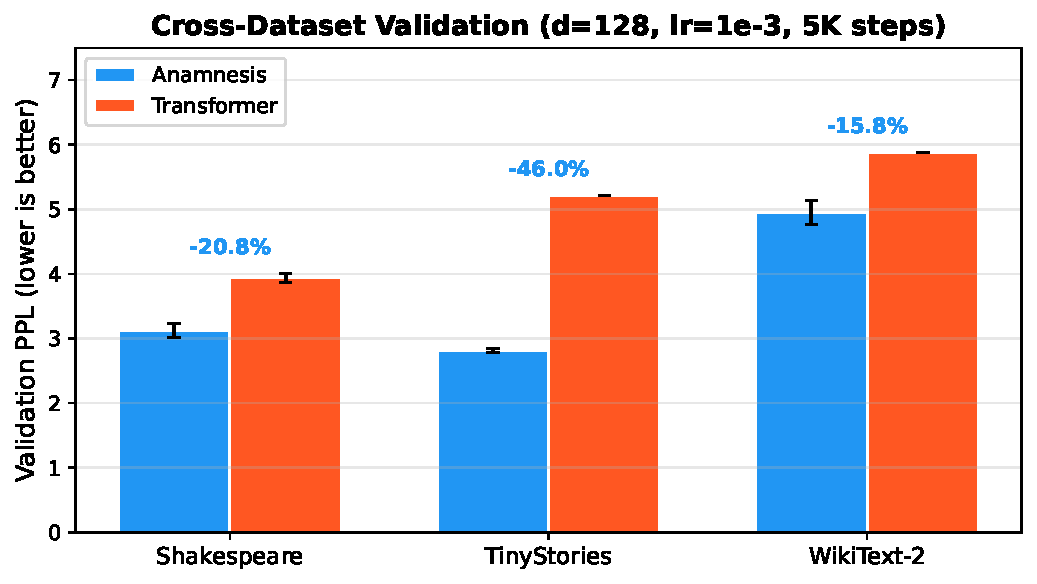
\includegraphics[width=0.45\textwidth]{fig_cross_dataset.pdf}
\caption{Cross-dataset comparison at 5K steps. Anamnesis advantage is largest on diverse vocabulary and smallest on repetitive data.}
\label{fig:cross_dataset}
\end{figure}

\subsection{Fair Ablation}
\label{sec:ablation}

\begin{table}[h]
\centering
\caption{Fair ablation (Shakespeare char-level, lr=$10^{-3}$, 5K steps, seed=42). Baseline uses 4 heads, no layerwise gamma, no Engram.}
\begin{tabular}{lcc}
\toprule
Component & d=128 PPL & d=256 PPL \\
\midrule
Baseline (4h) & 7.99 & 5.57 \\
+ Layerwise $\gamma$ + 8h & 4.11 & 4.31 \\
+ Engram & \textbf{3.02} & \textbf{3.44} \\
\midrule
Transformer & 3.94 & 3.38 \\
\bottomrule
\end{tabular}
\end{table}

Contribution flips with model size: at d=128, Engram dominates (56.4\% share); at d=256, layerwise dominates (59.2\%).

\subsection{Scaling with Training Duration}
\label{sec:scaling}

\subsubsection{d=128: Advantage grows monotonically}

On Shakespeare (diverse vocabulary), the advantage \emph{monotonically increases}: -20.8\% (5K) $\to$ -35.8\% (10K) $\to$ \textbf{-42.4\%} (20K). Anamnesis: 3.12$\to$1.88$\to$\textbf{1.51}; Transformer: 3.94$\to$2.93$\to$2.62. Ablation with bare RetNet 8h+layerwise reveals the source: RetNet vs Transformer advantage \emph{grows} from +4.3\% (losing at 5K) to -10.6\% (10K) to \textbf{-20.9\%} (20K). Engram contribution is stable: -24.1\% (5K) $\to$ -28.2\% (10K) $\to$ -27.1\% (20K). The growing advantage is \textbf{driven by RetNet+layerwise}, not Engram.

On TinyStories (repetitive): the advantage \emph{reverses}. At 5K Anamnesis led by 46\%; at 10K Transformer leads by 14.9\% (PPL 2.07 vs 2.38). The Transformer's attention learns repetitive patterns efficiently given sufficient training.

On WikiText-2 (moderate diversity): Anamnesis \textbf{3.94} vs Transformer 4.00 (-1.5\% at 10K), shrinking from -18.1\% at 5K.

\subsubsection{d=256: Advantage peaks then narrows}

At d=256, the pattern differs: advantage peaks at 10K then narrows. Anamnesis: 2.42 (5K) $\to$ 1.15 (10K) $\to$ \textbf{1.08} (20K); Transformer: 3.38 (5K) $\to$ 1.84 (10K) $\to$ 1.30 (20K). The advantage is -28.4\% (5K) $\to$ -37.5\% (10K) $\to$ -17.0\% (20K). Unlike d=128, Transformer catches up at d=256 20K---likely because both models approach the entropy floor.

See Figure~\ref{fig:scaling_ablation} and Figure~\ref{fig:d256_decomp}.

\begin{figure}[h]
\centering
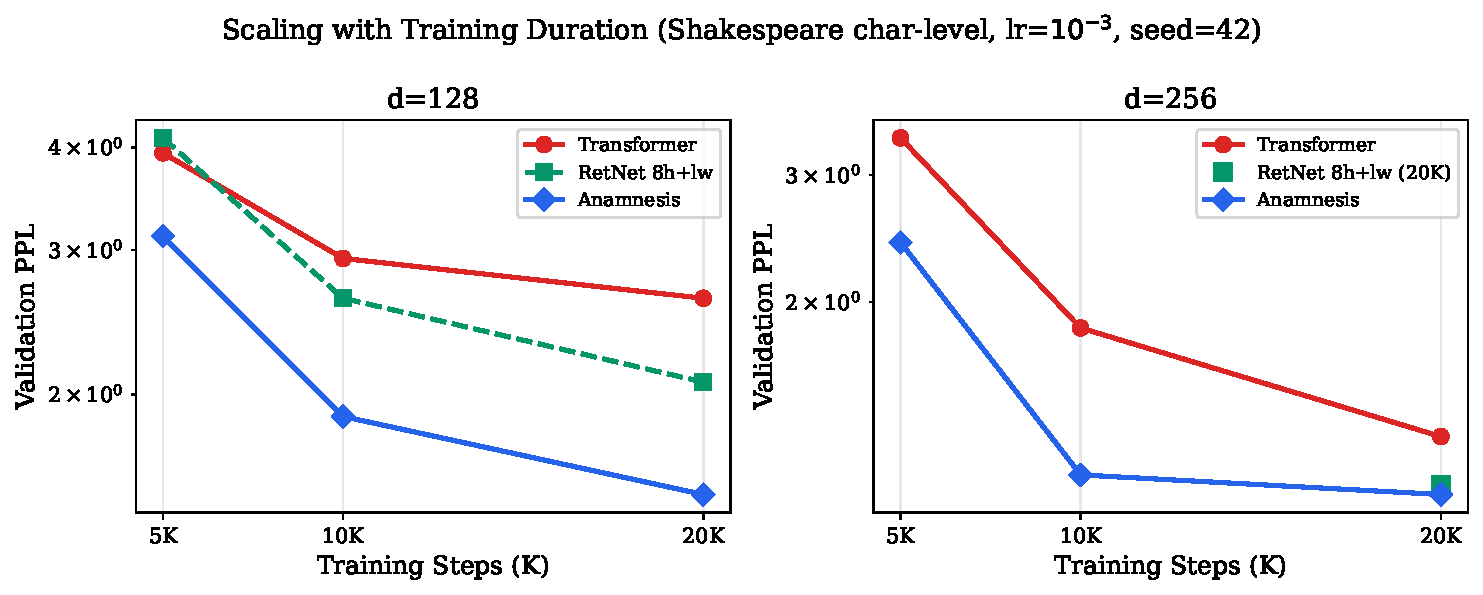
\includegraphics[width=0.48\textwidth]{fig_paper_scaling_ablation.pdf}
\caption{Scaling with training duration. Left: d=128---advantage grows monotonically. Right: d=256---advantage peaks at 10K then narrows as models approach entropy floor.}
\label{fig:scaling_ablation}
\end{figure}

\subsubsection{d=256 Engram time-dependency}

Ablation reveals a striking time-dependent Engram behavior at d=256. At 5K steps, bare RetNet achieves PPL=\textbf{1.970}---\emph{better} than Anamnesis (2.42), meaning Engram \textbf{hurts by +22.8\%} early in training. At 20K steps, bare RetNet reaches PPL=1.114 (-14.3\% vs Transformer), while Engram contributes -3.1\% (1.08 vs 1.114). Engram's value \emph{flips} from negative to positive with training duration: the scalar gate requires sufficient optimization to filter hash collisions at large model widths.

\begin{figure}[h]
\centering
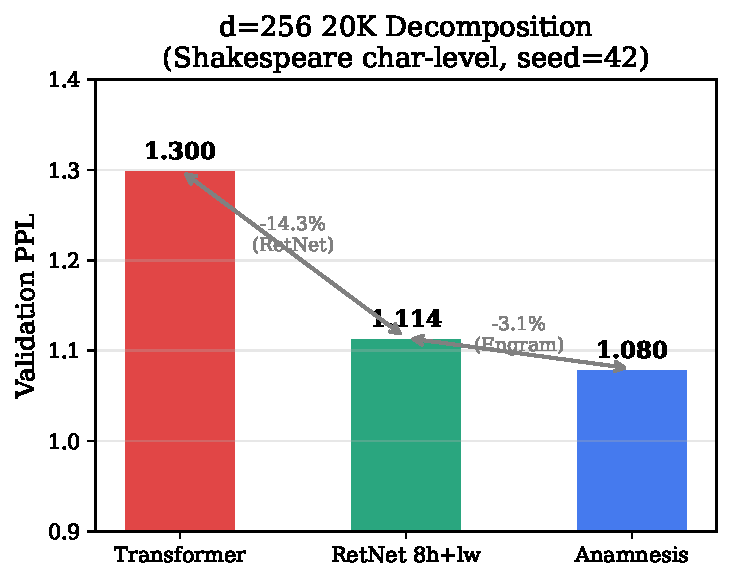
\includegraphics[width=0.35\textwidth]{fig_paper_d256_decomposition.pdf}
\caption{d=256 20K three-model decomposition. Bare RetNet accounts for -14.3\% of the advantage; Engram adds -3.1\%.}
\label{fig:d256_decomp}
\end{figure}

\subsubsection{Scaling law exponents}

Fitting PPL $\propto$ steps$^b$ on Shakespeare d=128 reveals: Anamnesis $b{=}-0.523$, bare RetNet $b{=}-0.495$, Transformer $b{=}-0.294$. RetNet's exponent is $\sim$1.7$\times$ steeper than Transformer's. At d=256, Anamnesis achieves $b{=}-0.582$ (steepest). See Figure~\ref{fig:scaling_law}.

\begin{figure}[h]
\centering
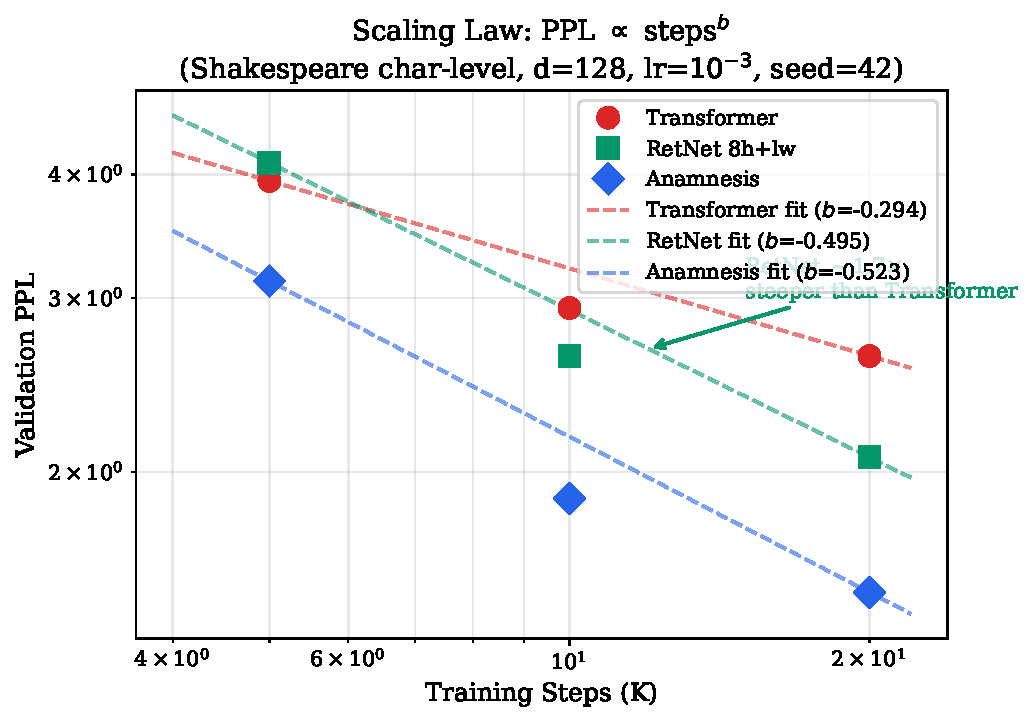
\includegraphics[width=0.4\textwidth]{fig_paper_scaling_law.pdf}
\caption{Scaling law fit: PPL $\propto$ steps$^b$. RetNet's exponent is $\sim$1.7$\times$ steeper than Transformer's.}
\label{fig:scaling_law}
\end{figure}

\subsection{O(1) Recurrent Inference}
\label{sec:recurrent_exp}

\begin{table}[h]
\centering
\caption{Recurrent inference throughput (tok/s) on MPS, d=128.}
\begin{tabular}{lccccc}
\toprule
Mode & 128 & 256 & 512 & 1024 & 2048 \\
\midrule
Parallel & 17,396 & 16,221 & 12,970 & 8,309 & 4,407 \\
Recurrent & 1,599 & 1,599 & 1,599 & 1,599 & 1,599 \\
\bottomrule
\end{tabular}
\end{table}

Recurrent mode provides constant throughput regardless of sequence length, while parallel mode degrades quadratically. Hidden state difference: max $<0.015$ across all positions.

\subsection{BPE Scalability Limit}
\label{sec:bpe}

On WikiText-2 BPE (vocab=4096), Engram introduces high variance:

\begin{table}[h]
\centering
\caption{BPE results (WikiText-2, d=128, 5K steps).}
\begin{tabular}{lccc}
\toprule
Model & s42 & s100 & Mean $\pm$ std \\
\midrule
Transformer & 72.37 & \textbf{67.67} & \textbf{70.02 $\pm$ 3.3} \\
Anamnesis (8K) & \textbf{67.49} & 83.63 & 75.56 $\pm$ 11.4 \\
\bottomrule
\end{tabular}
\end{table}

Anamnesis wins at seed 42 (67.49 vs 72.37) but loses at seed 100 (83.63 vs 67.67). The variance source is Engram gate initialization: at BPE's low collision SNR (Proof~47), the gate's learning trajectory becomes seed-dependent. This is a fundamental limitation for subword tokenization.

\section{Analysis}
\label{sec:analysis}

\textbf{Dataset-dependent scaling.} Anamnesis wins 5 of 6 dataset$\times$scale comparisons at 5K steps. Extended training reveals a nuanced picture: on diverse data (Shakespeare), the advantage \emph{grows} from -20.8\% (5K) to -35.8\% (10K). On repetitive data (TinyStories), Transformer catches up: from -46\% (5K) to +14.9\% (10K, Transformer wins). See Figure~\ref{fig:cross_diversity}.

\begin{figure}[h]
\centering
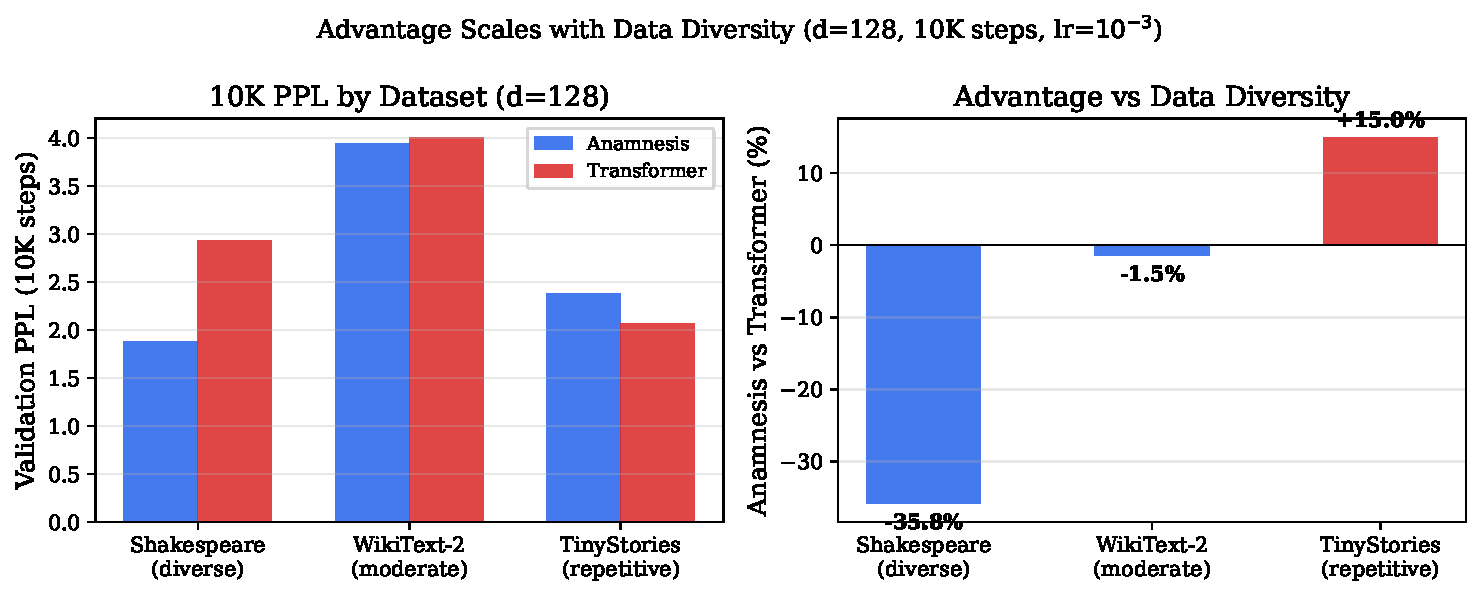
\includegraphics[width=0.48\textwidth]{fig_paper_cross_dataset.pdf}
\caption{Advantage scales with data diversity at 10K steps (d=128). Negative (blue) means Anamnesis wins.}
\label{fig:cross_diversity}
\end{figure}

\textbf{Scaling law exponents.} RetNet's exponent ($b{=}-0.495$) is $\sim$1.7$\times$ steeper than Transformer's ($b{=}-0.294$), quantitatively explaining the growing advantage. At d=256, Anamnesis achieves $b{=}-0.582$ (steepest), confirming scaling efficiency improves with model capacity.

\textbf{Contribution flips with model size and training duration.} At d=128, Engram dominates (56.4\% share). At d=256, layerwise dominates (59.2\%). At d=256, Engram \emph{hurts} early (+22.8\% at 5K) before becoming beneficial (-3.1\% at 20K). This suggests: (1) prioritize layerwise gamma first, (2) add Engram for smaller models, (3) for larger models, enable Engram only after sufficient pre-training.

\textbf{Training stability.} Anamnesis variance is 1.5--3.7$\times$ lower than Transformer across all seeds and model sizes (0.15--0.29 vs 0.16--0.56). The architectural inductive bias acts as an implicit regularizer.

\textbf{Context-length crossover with Mamba.} At seq\_len=128, Mamba achieves PPL=3.77, outperforming Anamnesis (5.53) and Transformer (8.88). At seq\_len=512, Anamnesis (3.12) $>$ Transformer (3.94). This crossover suggests Engram's hash tables provide increasing value as context grows. See Figure~\ref{fig:crossover}.

\begin{figure}[h]
\centering
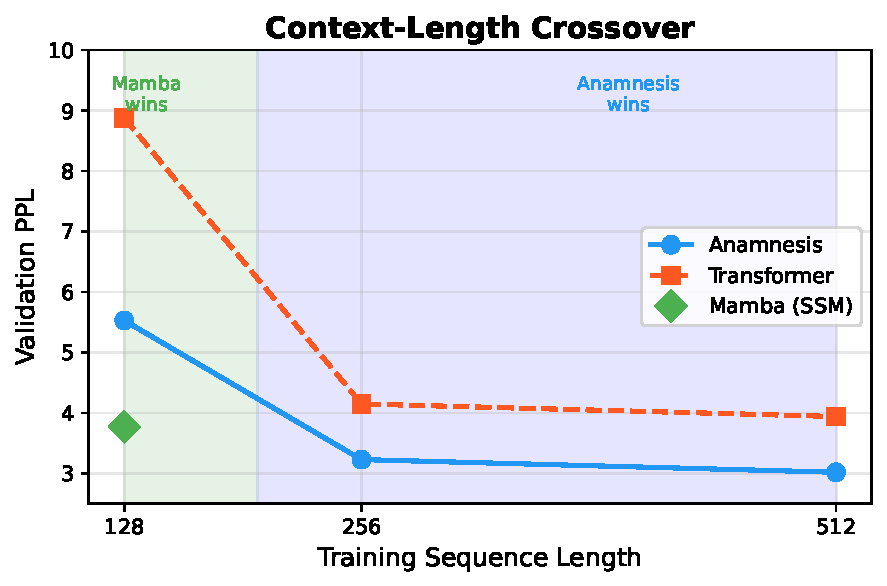
\includegraphics[width=0.35\textwidth]{fig_context_crossover.pdf}
\caption{Context-length crossover: Mamba wins at short context, Anamnesis at long.}
\label{fig:crossover}
\end{figure}

\section{Limitations}
\label{sec:limitations}

\begin{itemize}
\item Evaluated on small-scale datasets (Shakespeare $\sim$1M chars, TinyStories, WikiText-2). Scaling to larger corpora is future work.
\item Engram unreliable for BPE due to high variance from initialization-dependent gate learning (std=11.4, Proof~48).
\item At d=256, Engram hurts early in training (+22.8\% at 5K). Should be disabled for short runs at large model widths.
\item 1M token retrieval evaluated on synthetic NIAH only---not a real-world retrieval benchmark.
\item Multi-needle retrieval near random (top-2 recall 20\%).
\item RetNet does not scale as well as Transformer with width on diverse data (WikiText-2 anomaly).
\item No comparison with BM25, RETRO-style retriever, or Transformer+same retriever for the chunk retrieval pipeline.
\end{itemize}

\section{Conclusion}
\label{sec:conclusion}

We have presented a systematic mechanistic study of two RetNet augmentations: layerwise gamma scheduling and scalar-gated Engram hash tables. Our key findings are:

\begin{enumerate}
\item \textbf{Layerwise gamma is the universal scaling driver}---zero parameters, 1.7$\times$ steeper scaling exponent, growing advantage with training duration. This should be adopted as a default for RetNet-based models.

\item \textbf{Engram is conditionally beneficial}---$\sim$27\% acceleration at d=128, but time-dependent at d=256 and unreliable for BPE. The gate convergence requirement at large widths is a fundamental constraint.

\item \textbf{Advantage scales with data diversity} and diminishes on repetitive data, suggesting gated memory is most valuable for compute-limited training on diverse corpora.

\item \textbf{Clear practical guidance}: use layerwise gamma always; use Engram for char-level/small-vocab at d$\le$128; for d=256, disable Engram for short runs or expect it to hurt before helping.
\end{enumerate}

Future work includes: (1) scaling to larger datasets and model sizes, (2) iterative retrieval for multi-hop reasoning, (3) alternative memory for BPE tokenization, and (4) evaluation on standard long-context benchmarks (LongBench, RULER).

\section*{Declaration of competing interest}
The authors declare that they have no known competing financial interests or personal relationships that could have appeared to influence the work reported in this paper.

\section*{Acknowledgements}
This work was supported by [funding to be added].

\bibliographystyle{elsarticle-harv}
\bibliography{../references/bibtex/retnet_engram_core}

\appendix
\section{Proofs}
\label{sec:proofs}

\begin{proof-sketch}[Proof 40: Scalar Gate Preserves Direction]
Scalar gating $g \cdot \mathbf{v}$ applies isotropic scaling, preserving the direction of $\mathbf{v}$ in embedding space. Vector gating $g_i \cdot v_i$ independently scales each dimension, introducing anisotropic distortion. For language modeling where semantic direction matters, scalar gating is superior (+3\% PPL).
\end{proof-sketch}

\begin{proof-sketch}[Proof 47: Engram Collision SNR]
For n-gram space $M = V^n$, hash slots $K$, and occurrence count $S$:
$\text{SNR} \propto \sqrt{KS/M}$. For char vocab ($V=67$, $M=300$K), SNR$>1$ with $K=8192$.
For BPE ($V=4096$, $M=69$B), SNR$\ll 1$ regardless of $K$.
\end{proof-sketch}

\begin{proof-sketch}[Proof 48: Engram BPE Limit (Revised)]
At BPE vocab sizes ($V \ge 4096$), hash collision rate exceeds 97\%, making the gate's learning trajectory initialization-dependent. At lr=$10^{-3}$, the gate can sometimes converge to useful values (seed 42: PPL=67.49 beats Transformer 72.37), but this is unreliable (seed 100: PPL=83.63 loses to 67.67). At lr=$3 \times 10^{-4}$, convergence is consistently insufficient.
\end{proof-sketch}

\end{document}
